\chapter{Filtry cząsteczkowe}
%\subsection{Pojęcia podstawowe}
W tym rozdziale został opisany podstawowy algorytm filtra cząsteczkowego, wraz z jego adaptacją do wyznaczania lokalizacji. Ponadto opisano tutaj kilka wybranych usprawnień i modyfikacji podstawowej wersji.
\section{Opis problemu}
Celem filtru cząsteczkowego jest wyznaczenie rozkładu zmiennej stanu $X_k$, na podstawie szczątkowych pomiarów $Y_k$ za pomocą filtracji Bayesowskiej. \\
\begin{equation*}
\begin{tikzcd}
	X_0 \arrow{r} \arrow{d} &X_1 \arrow{r} \arrow{d} &X_2 \arrow{r} \arrow{d} &X_3\arrow{r} \arrow{d} &...\\
	Y_0 &Y_1 &Y_2 &Y_3 &...
\end{tikzcd} 
\end{equation*}
System taki, można opisać w następujący sposób
\begin{equation*}
	\begin{aligned}
		X_k=g(X_{k-1})+W_{k-1} \\
		Y_k=h(X_k)+V_k
	\end{aligned}
\end{equation*}
gdzie $g$ i $h$ to znane funkcje, a $W_{k-1}$ i $V_k$ to szumy. Jeśli oba szumy byłyby z rozkładu normalnego, a $g$ i $h$ są liniowe, to problem można rozwiązać za pomocą filtru Kalmana. Aby zyskać na ogólności, system można opisać w następujący sposób:
\begin{equation} \label{problem_eq}
	\begin{aligned}
		X_k=g(X_{k-1}, W_{k-1}) \\
		Y_k=h(X_k, V_k)
	\end{aligned}
\end{equation}
Taki problem, gdy funkcje $g$ i $h$ mogą być nieliniowe względem $X_k$, $Y_k$ oraz szumów $W_{k-1}$ i $V_k$, zazwyczaj jest zbyt złożony aby można było zastosować podejścia oparte o filtr kalmana. W takich przypadkach jedną z możliwości jest zastosowanie filtrów cząsteczkowych. Warto zauważyć, iż funkcja $g$ zawiera informacje o sterowaniu.
\section{Matematyczny opis filtracji Bayesowskiej}
Ogólne wzory na filtrowanie Bayesowskie można znaleźć na przykład na wikipedi \cite{wiki_bayes_filter}. Celem pojedynczego kroku filtracji jest wyznaczenie rozkładu a posteriori $p(X_{k}|Y_{0...k})$ opisującego prawdopodobieństwo, że system jest w stanie $X_k$, przy założeniu historii pomiarów $Y_{0...k}$, na podstawie rozkładu a priori $p(X_{k-1}|Y_{0...k-1})$ uzyskanego w poprzednim kroku oraz nowego pomiary $Y_k$. Etap predykcji można opisać poniższym równaniem:
\begin{equation} \label{evolution}
	p(X_k|Y_{0...k-1})=\int p(X_k|X_{k-1})p(X_{k-1}|Y_{0...k-1}) dX_{k-1}
\end{equation}
gdzie $p(X_k|X_{k-1})$ opisuje ewolucję systemu między krokami $k-1$ i $k$. Etap korekcji realizuje się w oparciu o wzór Bayesa, po otrzymaniu kolejnego pomiaru $Y_k$:
\begin{equation}\label{bayes_formula}
	p(X_k|Y_{0...k})=\frac{p(Y_k|X_k)p(X_k|Y_{0...k-1})}{p(Y_k|Y_{0...k-1})}
\end{equation}
gdzie $p(Y_k|X_k)$ opisuje rozkład prawdopodobieństwa uzyskania pomiaru $Y_k$ w stanie $X_k$. Warto zauważyć, iż $p(Y_k|Y_{0...k})$ można opisać wzorem:
\begin{equation}
p(Y_k|Y_{0...k})=\int p(Y_k|X_k)p(X_k|Y_{0...k-1}) dX_k
\end{equation}
więc mianownik równania \ref{bayes_formula} jest stały względem $X_k$. Mając to na uwadze, oraz podstawiając równanie \ref{evolution} do \ref{bayes_formula} można uzyskać ogólną formułę jednego kroku filtracji:
\begin{equation}
	p(X_k|Y_{0...k})=\mu p(Y_k|X_k)\int p(X_k|X_{k-1})p(X_{t-1}|Y_{0...t-1}) dX_{t-1}
\end{equation}
gdzie $\mu$ jest stałą normalizacyjną, pozostałą po przyjęciu że $p(Y_k|Y_{0...k})$ ma stałą wartość.
\section{Reprezentacja rozkładu prawdopodobieństwa}
Aby móc w praktyce zrealizować filtr cząsteczkowy, konieczne jest znalezienie sposobu na cyfrową reprezentację ciągłego rozkładu prawdopodobieństwa związanego ze stanem systemu. Robi się to przybliżając go za pomocą skończonego zbioru cząstek, gdzie każda cząstka wygląda w następujący sposób:
\begin{equation*}
	p_{i,k}=\{x_{k,i},w_{k,i}\}
\end{equation*}
gdzie $x_{k,i}$ to stan w iteracji $k$ związany z $i$-tą cząstką, $w_{k,i}$ to jej waga. Korzystając z takiej reprezentacji, rozkład $p(X_k|Y_{0...k})$ ze wzoru \ref{evolution} można zapisać w następujący sposób:
\begin{equation}
	p(x_k|Y_{0...k})\approx \sum_{i=0}^{N} w_{k,i}	\delta(X_k-x_{k,i})
\end{equation}
gdzie $N$ oznacza liczbę cząstek, a $\delta$ to delta Dirac'a. Dzięki takiej reprezentacji prawdopodobieństwo $p(X_k|Y_{0...k-1})$ opisane we wzorze \ref{evolution} zostaje zastąpione przez wagę $w_{k,i}$ dla każdej cząstki, co sprawia, że równanie \ref{bayes_formula} upraszcza się do:
\begin{equation}\label{weight_update}
	w_{k,i} = w_{k-1,i} p(y_k|x_{k,i})
\end{equation}

% Warto zauważyć, że taka reprezentacja realizuje procedurę importance sampling

\section{Podstawowy algorytm - SIR} \label{basic_algorithm}
Sam skrót SIR oznacza stochastic importance resampling, i jest to standardowa realizacja filtra cząsteczkowego w praktyce. Opis algorytmu można znaleźć w \cite{wiki_pf}. Sam importance sampling polega na wykorzystaniu właściwości jednego rozkładu prawdopodobieństwa, do próbkowania z drugiego. W tym przypadku, próbkujemy z rozkładu $p(X_k|Y_{0...k})$ korzystając $p(Y_k|X_k)$.
Algorytm SIR Przebiega w następujący sposób:
\begin{enumerate}[label=(\alph*)]
	\item Zaczyna się od zainicjowania zbioru cząstek losowymi stanami i równymi dla wszystkich cząstek wagami. Ważne jest, aby uzyskana w ten sposób populacja była w stanie odpowiednio oddać właściwości niezdyskretyzowanego rozkładu. \label{pf_init_step}
	
	\item Symuluje się ewolucję cząstek $x_{k-1,i}$, próbkując $x_{k,i}$ z rozkładu opisującego ewolucję systemu, $p(x_k|x_{k-1})$, obecnego w równaniu \ref{evolution}, a dobranemu na podstawie funkcji $g$ z równania \ref{problem_eq}. W praktyce ważne jest, aby rozkład $p(x_k|x_{k-1})$ uwzględniał szumy obecne w systemie, co sprowadza się do tego, że do ewolucji wprowadza cię trochę losowości. \label{pf_drift_step}
	
	\item Pojawia się nowy pomiar $y_k$, na podstawie którego na którego podstawie modyfikuje się wagi poszczególnych cząstek, korzystając z równania \ref{weight_update}. \label{pf_reweight_step}

	\item Wagi są normalizowane. \label{pf_weight_normalization_step}
	\begin{equation}
		w_{k,i}=\frac{w_{k,i}}{\sum_{j=0}^{N} w_{k,j}}
	\end{equation}

	\item Wyznacza się estymowany stan, wyznaczając ważoną średnią stanów wszystkich cząstek. Zazwyczaj jest to średnia ważona cząstek: \label{pf_est_step}
	\begin{equation}
		\hat{x_k} = \sum_{i=0}^{N} w_{k,i} x_{k,i}
	\end{equation}
	\item Przeprowadza się ponowne próbkowanie, generując nową populację cząstek z poprzedniej, korzystając z wag. W praktyce zazwyczaj nie przeprowadza się próbkowania co iterację, aby przyspieszyć obliczenia. Robi się to dopiero gdy spełnione jest pewne kryterium, którym najczęściej jest spadek efektywnej cząstek, opisanej równaniem \ref{neff_form} poniżej pewnego progu.
	\begin{equation}\label{neff_form}
		N_{eff_k} = \dfrac{1}{\sum w_{k,i}^2}
	\end{equation}
	Inne metody na określenie momentu próbkowania, można znaleźć na przykład w \cite{adaptive_resampling}.\label{resampling_step}
\end{enumerate}
\section{Adaptacja do wyznaczania lokalizacji}
Rozwiązanie problemu wyznaczania lokalizacji za pomocą filtra cząsteczkowego często jest nazywane lokalizacją Monte Carlo. Celem jest wtedy wyznaczenie pozycji i orientacji pewnego obiektu, na przykład robota. W takim przypadku rozkład $p(x_k|x_{k-1})$ opisuje model ruchu obiektu, natomiast pomiary $y_k$ są zebranymi danymi sensorycznymi. Prawdopodobieństwo $p(y_k|x_{k,i})$ wyznacza się na podstawie znanej mapy otoczenia.

\section{Przykład}\label{simple_example_chap}
Najprostszym przykładem problemu lokalizacji na którym można zademonstrować działanie filtra, jest ustalanie pozycji punktowego robota, przemieszczającego się ze stałą prędkością w kierunku ściany, mierząc swoją odległość od niej. Mapa w tym przypadku jest jednowymiarowa, a stan robota można opisać jedną liczbą zmiennoprzecinkową, mówiącą o jego pozycji. Pomiar $y_k$ jest odległością od robota do ściany na końcu drogi, natomiast jako rozkład $p(y_k|x_{k,i})$ przyjęto rozkład Gaussa. Na rysunku \ref{simple_example} przedstawiono efekt realizacji filtra cząsteczkowego. W tym przykładzie próbkowanie przeprowadzano na koniec każdej iteracji.

\begin{figure}[H]
	\begin{center}
		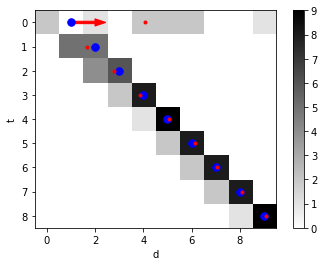
\includegraphics[width=10cm]{./simple_example.png}
		\caption{Przykładowa realizacja prostego filtra. Czerwona strzałka wskazuje kierunek ruchu robota, czerwone punkty pokazują estymowaną lokalizację robota, natomiast niebieskie punkty prawdziwe położenie. W kolejnych rzędach zestawiono histogramy położenia cząstek w poszczególnych iteracjach. Populacja składała się z 10 osobników.}\label{simple_example}
	\end{center}
\end{figure}

\section{Adaptacyjna liczba cząstek} \label{adaptive_chapter}
Oczywistym jest, że największy wpływ na złożoność obliczeniową filtra cząsteczkowego ma ilość cząstek. W \cite{adaptive} opisano algorytm który służy do dynamicznego zmieniania liczby cząstek. Polega on na zmodyfikowaniu kroku \ref{resampling_step} podstawowego algorytmu, gdzie tuż przed próbkowaniem wyznacza się nową liczbę cząstek. Wykonuje się to, kolejno usuwając cząstki, i sprawdzając o ile pogorszyła się jakość estymacji. Miarę tego pogorszenia mierzy się za pomocą funkcji opisanej poniższym równaniem
\begin{equation}\label{ceana_pogorszenia}
	\xi_t = |y_t-h(\hat{x_k})|
\end{equation}
i wyznacza się się je za każdym razem gdy usunie się cząstkę.

\begin{algorithm}[H]
	\SetAlgoLined
	\DontPrintSemicolon
	\caption{Algorytm dynamicznego doboru liczby cząstek.} \label{adaptive_N}
	Inicjalizacja $S_k=\{1,...,N_k\}$ i $K_k=\emptyset$\;
	Wyznaczenie $\xi(N_k)$\;
%	\begin{equation*}\text{Testowe usuwanie cząstek}\end{equation*}\;
	-------------------Testowe usuwanie cząstek\;
	\For{$d=0$ \KwTo $dim(x_{k,i})$}{
		Sortowanie indeksów cząstek S względem wymiaru $d$\;
		\For{$i \in S$}{
			\If{$||x_{k,i}^d-x_{k,i+1}^d||<\gamma_d$}{
				\begin{equation*}
					K_t = \begin{cases}
						K_t \cup \{i+1\} \text{ jeśli } w_{k,i}>w_{k,i+1}\\
						K_t \cup \{i\} \text{ w przeciwnym wypadku}
					\end{cases}\;
				\end{equation*}
				$S_t=S_t\slash K_t, n_s=dim\{S_t\}$\;
				$\hat{x_k} = \sum_{j \in S} w_{k,j} x_{k,j}$\;
				Wyznaczenie $\xi(n_s)$ ze wzoru \ref{ceana_pogorszenia} \;
			}
		}
	}

	-------------------Wyznaczanie nowego $N_k$\;
	\eIf{$\xi_k(n)>\alpha, \forall n \in [n_s,N_k]$}{
		$N_{k+1} \sim U(N_t,N_{max})$\;
	}{
		$N_{k+1}=argmin_n\{\xi(n)\}$ taki że $\xi(n)<\alpha$\;
	}
	\If{$N_{k+1}<N_{min}$}{
		$N_{k+1}=N_{min}$\;
	}
	
\end{algorithm}
W algorytmie \ref{adaptive_N} wydzielono dwie sekcje, testowe usuwanie cząstek oraz wyznaczanie nowego $N_k$. W pierwszym etapie wyznacza się wartości $\xi(n_s)$ dal różnych rozmiarów populacji, kolejno ujmując cząstki które leżą zbyt blisko siebie. Minimalna odległość na danym wymiarze $d$, po przekroczeniu której usuwa się jedną z cząstek, jest określana przez parametr $\gamma_d$. W drugim etapie wyznacza się nowy rozmiar populacji $N_{k+1}$ w zależności od $\xi_k$. Dopuszczalny błąd wprowadzany przez zmniejszenie populacji jest określany przez $\alpha$.

% Może się wydawać, iż zwiększy to złożoność obliczeniową, ponieważ trzeba o wiele więcej czasu poświęcić na analizę poszczególnych cząstek, jednak dzięki temu możemy zredukować samą ich liczbę, co sprawia, że koniec końców złożoność obliczeniowa nie zmienia się znacząco, a jakość wyników się poprawia
\section{Box Particle Filter} \label{bpf_chapter}
W tym podejściu zaproponowanym w \cite{bpf_base} i udoskonalonym w \cite{brbpf} zmieniono sposób reprezentacji cząstek. Zamiast punktów w przestrzeni stanów zastosowano interwały, w celu poprawy jakości estymacji w sytuacjach, gdy pomiary są zbyt szybkozmienne. Na przykład, dla problemu opisanego w podrozdziale \ref{simple_example_chap}, zamiast liczby rzeczywistej opisującej położenie robota, mielibyśmy odcinek na którym może się znajdować. Ponieważ zmianie ulega reprezentacja cząstek, wszystkie kroki algorytmu opisanego w rozdziale \ref{basic_algorithm} muszą zostać odpowiednio dostosowane.
\begin{itemize}
	\item W kroku \ref{pf_init_step}, cząsteczki interwałowe są inicjalizowane w taki sposób, aby pokrywać całą dopuszczalną przestrzeń stanów i nie nachodzić na siebie nawzajem.
	\item Ewolucja systemu opisana w kroku \ref{pf_drift_step}, zostaje zastąpione przez przekształcenie interwałów. Wykorzystuje się do tego funkcję interwałową $[g]$ konstruowaną na podstawie funkcji $g$ z równania \ref{problem_eq}. Ważne jest aby w przeciwieństwie do operacji z kroku \ref{pf_drift_step}, $[g]$ dawała w pełni deterministyczne wyniki, uwzględniające szumy obecne w systemie. Na przykład w problemie opisanym w rozdziale \ref{simple_example_chap}, jeśli cząstka byłaby interwałem [2,3] i miałaby być przesunięta o $1\pm 0.1$ to korzystając z reguły $3\sigma$ \cite{3_sigma_rule} można skonstruować nowy interwał po przesunięciu [2.9,4.1]. Opisuje się to następującym wzorem:
	\begin{equation}
		[x_{k+1,i}] = [g]([x_{k,i}])
	\end{equation}
	
	\item Zamiast pomiaru z kroku \ref{pf_reweight_step} wykorzystuje się interwał pomiarowy, uwzględniający jego niepewność (interwał ten można skonstruować według reguły $3\sigma$), oraz konstruując funkcję $[h]$, na podstawie funkcji $h$ z równania \ref{problem_eq}, generującą interwał pomiaru $[y]$ ze stanu danej cząstki. Nowe wagi ustala się na podstawie poniższych wzorów.
	\begin{equation}
		\begin{aligned}
			[z_{k,i}] = [h]([x_{k-1,i}])\\
			[r_{k,i}] = [z_{k,i}] \cap [y_{k}]\\
			w_{k,i} = \frac{|[r_{k,i}]|}{|[z_{k,i}]|} w_{k-1,i}
		\end{aligned}
	\end{equation}
	gdzie $[z_{k,i}]$ jest przewidywanym interwałem pomiaru dla cząstki $i$ w kroku $k$, $[y_{k}]$ jest interwałem faktycznie zmierzonego pomiaru, a $|\bullet|$ jest objętością interwału (dla przykładu z rozdziału \ref{simple_example_chap} byłaby to długość odcinka).
	\item Wagi są normalizowane tak samo jak w punkcie \ref{pf_weight_normalization_step} podstawowego algorytmu.
	
	\item Przed wyliczeniem estymowanego stanu można przeprowadzić zawężenie interwałów. Polega ono na pomniejszeniu $[x_{k,i}]$ w oparciu o interwał $[r_{k,i}]$. W przykładzie z rozdziału \ref{simple_example_chap}, mogło by to wyglądać w następujący sposób: jeśli uzyskano pomiar [7,9] który można uzyskać tylko w interwale [4,6], to cząstka z interwałem [3,5] zostanie zawężona do [4,5].
	
	\item Estymacja stanu odbywa się z wykorzystaniem średniej ważonej centrów interwałów (dla przykładu z rozdziału \ref{simple_example_chap} byłby to środek odcinka).
	\begin{equation}
		\hat{x_k} = \sum_{i=0}^{N} w_{k,i} C_{k,i}
	\end{equation}
	gdzie $C_{k,i}$ jest centrum $i$-tej cząstki w $k$-tej iteracji.
	\item Przed próbkowaniem można sprawdzić, czy cząstki nie nachodzą na siebie nawzajem za bardzo. Robi się to korzystając ze wzoru
	\begin{equation}
		\begin{aligned}
			\theta = \sqrt{\frac{\sum_{i=0}^{N}|[x_{k,i}]|}{N |P_{union}|}}
		\end{aligned}
	\end{equation}
	gdzie $P_{union}$ jest najmniejszym interwałem który zawiera wszystkie interwały $[x_{k,i}]$. Gdy $\theta$ jest większe niż pewien próg, populacja jest inicjalizowana na nowo równomiernie dzieląc $P_{union}$.
	
	\item Ponowne próbkowanie przebiega zupełnie inaczej niż w kroku \ref{resampling_step} podstawowego. Sam moment ponownego próbkowania można nadal dobierać według wzoru \ref{neff_form}. Próbkowanie zostaje zastąpione podziałem wybranych cząstek. Dla przykładu, gdy dana cząstka po próbkowaniu powinna być wzięta pięć razy, zostaje ona pięć razy podzielona wzdłuż najdłuższego wymiaru (może też być dzielona wzdłuż losowo wybranego interwału).
	\item Jednym z najważniejszych usprawnień zaproponowanych w \cite{brbpf} jest reinicjalizacja cząstek, w przypadku gdy suma wag spadnie do zera. Jest to konieczne, ponieważ w takim przypadku niemożliwe staje się próbkowanie.
\end{itemize}

\section{Wprowadzenie operatora mutacji} \label{evol_chap}
W \cite{pfgen} zaproponowano, aby wzbogacić proces próbkowania z kroku \ref{resampling_step} podstawowego algorytmu o operatory krzyżowania i mutacji. W kontekście wyznaczania lokalizacji, krzyżowanie można zaimplementować jako liniową interpolację dwóch losowo wybranych cząstek, natomiast mutację jako niewielkie zaszumienie cząstek. Pozwala to na poprawę działania filtra przy bardzo powolnej ewolucji, bądź nawet jej braku.
